\chapter{Analyse  Et Calcul  D’une Loi De Commande  Par Retour  D’état }
\addcontentsline{toc}{chapter}{Analyse  Et Calcul  D’une Loi De Commande  Par Retour  D’état }
 \section{Le modèle linéarisé est-il commandable?}
 En calculant la matrice de commandabilité $Co$ tel que : \\\\
 $Co=[B\quad AB \quad A^{2}B]$\\
 et on trouve :\\\\
 
 $Co=\begin{bmatrix} 
64.9351 & -0.5975 & 0.0110 \\
0 & 0.5975 & -0.0173 \\
0 & 0 & 0.0064  
\end{bmatrix}$\\\\\\
 
On alors le $rang(Co)=3$ est qui est égale a la dimention du système, d'ou le système est commandable.\\  
De même si on va le vérifier avec MATLAB  \hyperref[section1.1]{(voir Annexe)}\label{annexe1}\\
 
 
 
 
 \section{Calcule Des Valeurs Des Gains K et N Permettant De Remplir L’ensemble Des Conditions.}
 
\begin{center}
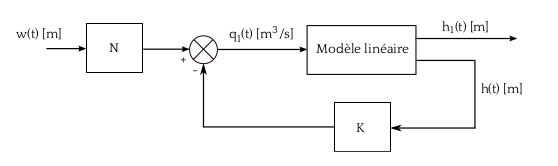
\includegraphics[scale=0.5]{fig2.png}
\captionof{figure}{\textit{ Retour d’état.}}
\label{fig2} 
\end{center}


